\newpage	
\def \currentAuthor {Florian Tipotsch}
	\section{Technologie für Webapp}
\begin{itemize}
	\item PHP - Für Webapp
	\item Html - Für Webapp 	
	\item MySql - Für Datenbanken
	\item \nameref{sec:YII2} - Für Webapp
	\item \nameref{sec:MVC} - Für Webapp
	\item \nameref{sec:CRUD} - Für Webapp
	\item REST - Für Datenbank, Webapp und Datenspeicherung
\end{itemize}
	\subsection{HTML - Hypertext Markup Language}
	HTML sind die Grundlagen für jede Website. Sie bilden die Grundstruktur jeder Webseite, und werden von Browsern dargestellt. HTML wird von dem World Wide Web Consortium (W3C) \cite{W3C} und dem Web Hypertext Application Technology Working Group (WHATWG) \cite{WHATWG} weiterentwickelt.
	
	Gute Ressourcen zum lernen und schreiben von HTML findet man auf w3schools.com \cite {W3schools}
	
	\subsection{Was ist Yii}
	Yii ist ein high Performance PHP Framework welches vor allem für die Entwicklung im Web2.0 eingesetzt wird. Web 2.0 fördert das User aktiv im Web mitmachen. Diese können eigenen Beiträge erstellen und diese auf der Website anzeigen lassen. Mehr dazu im Kapitel \nameref{sec:YII2}\cite{Web_2}

	\subsubsection{Alternative zu Frameworks}
	Yii kann sehr weitreichend eingesetzt werden. Mit dem richtigen Wissen und Fähigkeiten kann man alles was mit einer PHP Seite möglich ist in Yii2 umsetzten.

Allerdings sind Frameworks nicht Administratoren freundlich da sie sehr viel Vorwissen erfordern um diese richtig zu implementieren und zu warten. Einfacher zu implementieren sind CMS Systeme. Es gibt sehr viele Große CMS Systeme zum Beispiel:

\begin{itemize}
\item Joomla
\item Wordpress
\item Drupal
\item Contao
\end{itemize}

Diese haben wir auch schon im Unterricht kennengelernt und damit Websites erstellt. Vorteile sind vor allem die einfache Implementierung und rasche Einrichtung einer Website. Auch SEO wird von den CMS Systemen vereinfacht. Nachteile sind allerdings oft eingeschränkte Möglichkeiten und grenzen welches das CMS setzt.

\subsubsection{Warum haben wir uns für YII2 entschieden}

Der Hauptgrund warum wir uns gegen CMS Systeme entschieden haben sind die eingeschränkten Möglichkeiten die wir damit hätten. Bei YII2 können wir die gesamte Website nach unseren Bedarf zusammenstellen und auch so bearbeiten wie wir es wollen. Es war uns auch wichtig das wir nach modernen Entwurfsmustern arbeiten. Bei Yii2 wird das \nameref{sec:MVC} Muster eingesetzt.

Wir hätten uns auch für andere Frameworks entscheiden können allerdings war uns Yii2 schon bekannt und wir haben damit schon einige Websites erstellt.

Alternativen für Yii2 sind:

\begin{itemize}
	\item PureMVC
	\item Laravel
\end{itemize}

\subsection{PureMVC}
PureMVC ist seit dem Release in 2008 unverändert. Das hat den Vorteil das der administrative aufwand sehr gering ist aufgrund nicht vorhandener Updates. Außerdem muss man das Framework nur einmal lernen und kann dieses dann meistern ohne irgendwelche Änderungen zu befürchten.
Es gibt auch Best-Practicse Beispiele in vielen verschiedenen Sprachen. Diese findet man auf der Website. \cite{Pure_MVC}

\subsection{Laravel}
Laravel: PHP That Doesn’t Hurt. Code Happy and Enjoy The Fresh Air.
Laravel will PHP einfach und übersichtlich Programmierbar machen dazu verwendet es auch das MVC Muster und auch den PHPComposer um sehr einfach neue Erweiterungen zu installieren. Auch bei Laravel gibt es sehr gute Documentationen. Diese findet man auf der Website. \cite{laravel}


\newpage
\def \currentAuthor{Kevin Glatz}


\section{Technologien für die Datenauslesung}

\begin{itemize}
	\item Gas Sensor - Für Luftqualität
	\item Wärmesensor - Für Raumtemperatur	
	\item Luftfeuchtigkeit - Für Luftqualität
	\item Schalter - Für Futtermenge
	\item kinetischer Motor - für geregelte Luftzufuhr
	\item WLAN - Für Datenübertragung

\end{itemize}

\subsection{Gas Sensoren}
Für die Auswertung der Gaswerte stehen uns mehrere Module zur Verfügung.  Zum einen stand uns die vielfältige MQ-Serie zur Verfügung oder der spezialisierter CCS811 von Adafruit. 

In der Schule haben wir nicht nur den MQ2 Sensor zur Verfügung bereitgestellt bekommen, sondern auch den Adafruit CCS811. Wir bedanken uns dafür vielmals.

\subsubsection{MQ Gas Sensoren}

\begin{itemize}
\item {MQ2}
	Methane, Butane, LPG, smoke
\item {MQ3}
	Alcohol, Ethanol, smoke
\item {MQ4}
	Methane, CNG Gas
\item {MQ5}
	Natural gas, LPG
\item {MQ6}
	LPG, butane gas
\item {MQ7}
	Carbon Monoxide
\item {MQ8}
	Hydrogen Gas
\item {MQ9}
	Carbon Monoxide, flammable gasses
\item Mehr gibt es auf der Website: \cite{MQ_Sensoren}
\end{itemize}



{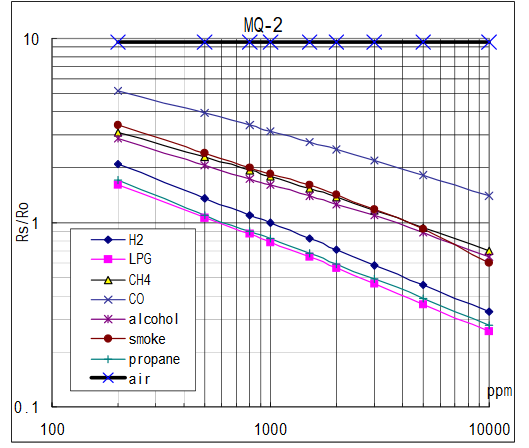
\includegraphics[width=0.8\linewidth]{figures/DatasheetMQ2.png}}{\cite{MQ_Datasheet}}

\cite{MQ_Sensoren}
\newline 

Im Datasheet \cite{MQ_Datasheet} kann man herauslesen das der Sensor MQ2 \cite{MQ_Sensoren} H2, LPG, CH4, CO, Alkohol, Rauch und Propan in einem Bereich von 200 bis 10000 Parts per million (Anteil pro Million) messen kann. Wie empfindlich der Sensor ist, hängt von den RS und RO werten ab.

\begin{itemize}
	\item RS: Sensor Widerstand bei verschiedenen Konzentrationen von Gas
	\item RO: Sensor Widerstand bei 1000ppm von H2 bei sauberer Luft.
\end{itemize}

Da der MQ-2  auf so viele Gase außer Co2 reagiert haben wir uns entschlossen eine Alternative zu suchen. Glücklicherweise hat uns die Schule auch den CCS811 von Adafruit zur Verfügung stellen können,

\subsubsection{Adafruit CCS811}

In unserem Projekt haben wir uns letztendlich für den CCS811 von Adafruit entschieden. Im Gegensatz zu dem MQ-Sensoren erlaubt der CCS811 eCO2 in einem Bereich von 400 bis 8192 ppm (parts per million) auszulesen. 
\cite{CCS811man}

Dadurch können wir uns komplizierte mathematische Formelrechnungen sparen und direkt den gewünschten Datentypen verwenden.

\subsection{Wärmesensor}

\subsubsection{DHT11}

In dem Arduino Uno Set war der DHT 11 Wärme und Temperatur Sensor von Adafruit direkt mitgeliefert. Dieses Modul erlaubt es uns digitale Daten in einem zwei Sekunden Takt auszulesen. Es liest die Wärme in einem Bereich von 0 bis 50°C, die Daten können allerdings um etwa 2°C variieren.

\subsubsection{CCS811}

Der CCS811 besitzt auch einen Thermistor, mit welchem wir direkt die Raumtemperatur auslesen können. Da der DHT11 allerdings auch die Luftfeuchtigkeit anzeigen kann, verwendeten wir diesen anstatt den CCS811. 
\cite{CCS811man}

\subsection{Luftfeuchtigkeit}

Da der DHT direkt bei dem Arduino Kit mit dabei war, gab es keinen Grund einen anderen Sensor zu suchen. Das Modul erlaubt uns die Luftfeuchtigkeit in einem Bereich von 20 bis 80 Prozent zu messen. Diese Daten können allerdings um beinahe 5\% variieren.  

\subsection{kinetischer Motor}

Für eine automatisierte Luftzufuhr verwenden wir den Servo-Mikrocontroller SG90. Sowie der DHT 11 war dieser Motor schon im Arduino Uno Set beigelegt. Der 3-polige Servo wird für die Luftzufuhr verwendet. Der Propeller am drehenden Motor öffnet und schließt die Luftklappe des Kastens. Das ermöglicht eine höhere Kontrolle und Regulierung des CO2 Wertes. (https://servodatabase.com/servo/towerpro/sg90)

\subsection{Hebel}

Um zu sehen wie viel Futter für die Insekten vorhanden ist, verwendeten wir einen Joystick. Dieser Joystick war beim Arduino Uno Set mitgeliefert und kann die X- und Y-Achse ablesen sowie auf Druck zu reagieren. Anhand der Y-Achse kann man den Joystick als Hebel verwenden um den momentanen Futterstand abzulesen. 


\subsection{Datenübertragung}

Damit der Nutzer die Daten letztendlich auf der Website abrufen kann, verwenden wir das WLAN-Modul ESP8266. Dieser sehr beliebter und billiger Mikrocontroller fungiert als eine voll Funktionsfähige Netzwerkschnittstelle. Es erlaubt uns auch den Brutkasten kabellos und benutzerfreundlicher zu Gestalten
